%%
%% Copyright 2007, 2008, 2009 Elsevier Ltd
%%
%% This file is part of the 'Elsarticle Bundle'.
%% ---------------------------------------------
%%
%% It may be distributed under the conditions of the LaTeX Project Public
%% License, either version 1.2 of this license or (at your option) any
%% later version.  The latest version of this license is in
%%    http://www.latex-project.org/lppl.txt
%% and version 1.2 or later is part of all distributions of LaTeX
%% version 1999/12/01 or later.
%%
%% The list of all files belonging to the 'Elsarticle Bundle' is
%% given in the file `manifest.txt'.
%%
%% Template article for Elsevier's document class `elsarticle'
%% with harvard style bibliographic references
%% SP 2008/03/01
%%
%%
%%
%% $Id: elsarticle-template-harv.tex 4 2009-10-24 08:22:58Z rishi $
%%
%%
\documentclass[preprint,authoryear,12pt]{elsarticle}

%% Use the option review to obtain double line spacing
%% \documentclass[authoryear,preprint,review,12pt]{elsarticle}

%% Use the options 1p,twocolumn; 3p; 3p,twocolumn; 5p; or 5p,twocolumn
%% for a journal layout:
%% \documentclass[final,authoryear,1p,times]{elsarticle}
%% \documentclass[final,authoryear,1p,times,twocolumn]{elsarticle}
%% \documentclass[final,authoryear,3p,times]{elsarticle}
%% \documentclass[final,authoryear,3p,times,twocolumn]{elsarticle}
%% \documentclass[final,authoryear,5p,times]{elsarticle}
%% \documentclass[final,authoryear,5p,times,twocolumn]{elsarticle}

%% if you use PostScript figures in your article
%% use the graphics package for simple commands
%% \usepackage{graphics}
%% or use the graphicx package for more complicated commands
%% \usepackage{graphicx}
%% or use the epsfig package if you prefer to use the old commands
%% \usepackage{epsfig}

%% The amssymb package provides various useful mathematical symbols
\usepackage{graphicx}
\usepackage{epstopdf}
\usepackage{amssymb}
\usepackage{amsmath}
%\usepackage{a4wide}
\usepackage{color}
%\usepackage{subcaption}
\newcommand{\hilight}[1]{\colorbox{yellow}{#1}}
%% The amsthm package provides extended theorem environments
%% \usepackage{amsthm}
\newcommand\solidrule[1][1cm]{\rule[0.5ex]{#1}{1pt}}
\newcommand\dashedrule{\mbox{\solidrule[1mm]\hspace{1mm}\solidrule[1mm]\hspace{1mm}\solidrule[1mm]\hspace{1mm}}}

\newcommand{\ustar}{\ensuremath{U^{*}}}
\newcommand{\cstar}{\ensuremath{c^{*}}}
\newcommand{\reynoldsnumber}{\ensuremath{Re}}
\newcommand{\massstiff}{\ensuremath{\Pi_1}}
\newcommand{\massdamp}{\ensuremath{\Pi_2}}


\newcommand{\Tan}[1]{{\textcolor{blue}{{\bf{\it{ **Tan: #1 **}}}}}}
\newcommand{\JL}[1]{{\textcolor{red}{{\bf{\it{ **JL: #1 **}}}}}}

%% The lineno packages adds line numbers. Start line numbering with
%% \begin{linenumbers}, end it with \end{linenumbers}. Or switch it on
%% for the whole article with \linenumbers after \end{frontmatter}.
%% \usepackage{lineno}

%% natbib.sty is loaded by default. However, natbib options can be
%% provided with \biboptions{...} command. Following options are
%% valid:

%%   round  -  round parentheses are used (default)
%%   square -  square brackets are used   [option]
%%   curly  -  curly braces are used      {option}
%%   angle  -  angle brackets are used    <option>
%%   semicolon  -  multiple citations separated by semi-colon (default)
%%   colon  - same as semicolon, an earlier confusion
%%   comma  -  separated by comma
%%   authoryear - selects author-year citations (default)
%%   numbers-  selects numerical citations
%%   super  -  numerical citations as superscripts
%%   sort   -  sorts multiple citations according to order in ref. list
%%   sort&compress   -  like sort, but also compresses numerical citations
%%   compress - compresses without sorting
%%   longnamesfirst  -  makes first citation full author list
%%
%% \biboptions{longnamesfirst,comma}

% \biboptions{}

\journal{Journal of Fluid Structures}

\begin{document}
\begin{frontmatter}

%% Title, authors and addresses

%% use the tnoteref command within \title for footnotes;
%% use the tnotetext command for the associated footnote;
%% use the fnref command within \author or \address for footnotes;
%% use the fntext command for the associated footnote;
%% use the corref command within \author for corresponding author footnotes;
%% use the cortext command for the associated footnote;
%% use the ead command for the email address,
%% and the form \ead[url] for the home page:
%%
%% \title{Title\tnoteref{label1}}
%% \tnotetext[label1]{}
%% \author{Name\corref{cor1}\fnref{label2}}
%% \ead{email address}
%% \ead[url]{home page}
%% \fntext[label2]{}
%% \cortext[cor1]{}
%% \address{Address\fnref{label3}}
%% \fntext[label3]{}

\title{A study on the energy transfer of a square prism under fluid-elastic galloping}

%% use optional labels to link authors explicitly to addresses:
%% \author[label1,label2]{<author name>}
%% \address[label1]{<address>}
%% \address[label2]{<address>}

\author{H.G.K.G. Jayatunga, B.T. Tan, J. S. Leontini}

\address{}

\begin{abstract}
Extracting useful energy from flow induced vibrations has become a developing area of research in recent years. In this paper, we analyse power transfer of an elastically mounted body under the influence of aeroelastic galloping. The system and the power transfer is analysed by numerically integrating the quasi-steady state model equations. The power transfer is analysed for both high ($\reynoldsnumber=22300$) and low ($\reynoldsnumber=165$) Reynolds numbers cases, and the impact of the system mass is investigated for both.

At high mass ratios ($m^*>50$), the power transfer is completely controlled by galloping and essentially independent of the mass. A combined mass-damping coefficient, \massdamp, that can be derived from the equation of motion, is shown to be the parameter that governs power output. The system is a balance between the power delivered to the system due to hydrodynamic forcing and power removed through mechanical damping which are governed by the hydrodynamic forcing characteristics (i.e. the lift force as a function of incident angle) and mechanical damping coefficient respectively.  The peak efficiency of $0.26\%$ for $\reynoldsnumber=165$ and $6.7\%$ for $\reynoldsnumber=22300$ were observed when the non-dimensionalised mass-damping factor becomes 0.314 and 1.04 respectively.

A contradictory behaviour is observed at low $m^*$ between the low and high \reynoldsnumber\ cases. The forcing due to vortex shedding at low Reynolds numbers  suppresses the galloping excitation and results in a reduced power output. For the case with high \reynoldsnumber\ power output increases as $m^*$ is reduced . For this high \reynoldsnumber\ case, at low $m^*$ the reduction in inertia allows the body to accelerate faster and spend a larger portion of the period at relatively high transverse velocities. Extrapolating this trend, the limit to peak efficiency is found to be $13.5\%$ and occurs when $m^*\rightarrow 0$ and $\ustar \rightarrow \infty$ and $\massdamp=1.22$



\end{abstract}

\begin{keyword}
%% keywords here, in the form: keyword \sep keyword

%% MSC codes here, in the form: \MSC code \sep code
%% or \MSC[2008] code \sep code (2000 is the default)

\end{keyword}

\end{frontmatter}

% \linenumbers

%% main text
\section{Introduction} 

Fluid-elastic galloping is one of the sub-areas of research in fluid structure interactions. This area has been of interest due to the vibrations crated by galloping on transmission lines and civil structures and leading them to failure. Therefore understanding this phenomenon in order to suppresses these vibrations was quite important. However, the search for alternate energy sources with minimal environmental impact has become an important area of research in the modern word. Therefore researchers are moving towards investigating the possibility of extracting useful energy from this vibrations rather than suppressing them. Therefore, it is quite important to understand the governing parameters and analyse the influence of them on the energy transfer from the fluid to the body, because this understanding will lead to develop better practical applications. Therefore, in this paper we focus on understanding the energy transfer from the fluid to the body and isolate the governing parameters influencing it.

According to \citet{Paidoussis2010}, \citet{Glauert1919} provided a criterion for galloping by considering the auto-rotation of an aerofoil.  \citet{DenHartog1956} provided a theoretical explanation for galloping for iced electric transmission lines. A weakly non-linear theoretical aeroelastic model to predict the response of galloping was developed by \citet{Parkinson1964} based on the quasi-steady state hypothesis. Experimental lift and drag data on a fixed square prism at different angles of attack were used as an input for the theoretical model. It essentially used a curve fit of the transverse force to predict the galloping response. The study managed to achieve a good agreement with experimental data.














However, the QSS model equation when solved analytically using the sinusoidal solution method cannot predict the response for cases with low mass ratios. \citet{Joly2012} observed that finite element simulations show a sudden change in amplitude below a critical value of the mass ratio. The model equation defined in \citet{Parkinson1964} was modified to account for the vortex shedding and solved numerically to predict the reduced amplitude at low mass ratios to the point where galloping is no longer present. \citet{Barrero-Gil2010a} investigated the possibility of extracting power from vibrations caused by galloping using the quasi-steady state model. In the conclusions of that paper it was pointed out that in order to obtain a high power to area ratio, the mass-damping ($m^*\zeta$) parameter should be kept low. The same study investigated the influence of the characteristics of the $C_y$ curve on maximum power output.

Here, the modified QSS model developed by \citet{Joly2012} is integrated numerically for low Reynolds numbers. The focus is on the power extraction potential as a function of mechanical parameters (i.e. frequency of oscillation, damping factor and mass ratio). To this end, a series of previously mentioned mechanical parameters are tested at two different values of \reynoldsnumber: $\reynoldsnumber = 165$, a case that should remain laminar and essentially two-dimensional; $\reynoldsnumber = 22300$, a case where the flow is expected to be turbulent and three-dimensional. Both cases require the input of transverse force coefficients $C_y$ as a function of angle of attack $\theta$ for a fixed body. These data are provided from direct numerical simulations for the $\reynoldsnumber = 165$ case, while the data provided by \citet{Parkinson1964} are used for the $\reynoldsnumber = 22300$ case.

The structure of the paper is as follows. Section \ref{sec:theory} presents the modified QSS model, the method for the calculation of power output, and the parameters used. Section \ref{sec:results} presents the results, first of the fixed body tests at a range of $\theta$, then of the response characteristics predicted by the integration of the QSS model for both the high and low \reynoldsnumber\ cases. For the low \reynoldsnumber\ case, the results of the QSS model are compared to those of full direct numerical simulations of the fluid-structure interaction problem. Finally, section \ref{sec:conc} presents the conclusions that can be drawn from this work.
% % % % % % % % % % % % % % % % % % % % % % % % % % % % % % % % % % % % % % % % % % % % % % % % % % % % % % % % % % % % % % % % % % % % % % % % 
\section*{Nomenclature}
%\textbf{Nomenclature}

\begin{tabular}{ll}
$a_1,a_3,a_5,a_7$ & coefficients of the polynomial to determine $C_y$ \\ 
$A$ & displacement amplitude\\
$c$ & damping constant \\
$D$ & characteristic length (side length) of the cross section of the body \\
$f=\sqrt{k/m}/2\pi$ & natural frequency of the system \\
$F_y$ & instantaneous force normal to the flow \\ 
$F_0$& amplitude of the oscillatory force due to vortex shedding \\
$k$ & spring constant \\
$m$ & mass of the body \\
$m_a$ & added mass \\
$P_d$ & power dissipated due to mechanical damping  \\
$P_{in}=\rho U^3D/2$ & Energy flux of the approaching flow \\
$P_{mean}$ & mean power \\
$P_t$   & power transferred to the body by the fluid \\
$t$ & time \\
$U$ & freestream velocity \\
$U_i$ & Induced velocity \\
$y,\dot{y},\ddot{y}$ & transverse displacement, velocity and acceleration of the body \\
$\mathcal{A}=DL$ & frontal area of the body\\ 
$\lambda$ & Inverse time scale of a galloping dominated flow \\
$\lambda_{1,2}$ & Eigenvalues of linearized equation of motion \\
$\rho$ & fluid density  \\
$\omega_n= 2 \pi f$ & natural angular frequency of the system  \\
$\omega_s$ & vortex shedding angular frequency \\
$\cstar=cD/mU$ & non-dimensionalised damping factor \\
$C_y=F_y/0.5\rho U^2DL$ & normal (lift) force coefficient \\
$m^*=m/\rho D^2L$ & mass ratio \\
$Re$ & Reynolds number  \\
$U^*=U/fD$ & reduced velocity  \\
$Y=y/D$ & non-dimensional transverse displacement \\
$\dot{Y}=m^*\dot{y}/a_1U$ & non-dimensional transverse velocity \\
$\ddot{Y}=m^{*2}D/a_1^2U^2$ & non-dimensional transverse acceleration \\
$\Gamma_1 = 4\pi^2m^{*2}/U^{*2}a_1^2$ & First dimensionless group arising from linearised, non-dimensionalised equation of motion\\
$\Gamma_2 = c^*m^*/a_1$ & Second dimensionless group arising from linearised, non-dimensionalised equation of motion\\
$\zeta= c/2 m \omega_n$ & damping ratio \\
$\theta= \tan^{-1}{(\dot{y}/U)}$ & instantaneous angle of incidence (angle of attack)\\
$\massstiff =  4\pi^2m^{*2}/U^{*2}$ & Combined mass-stiffness parameter\\
$\massdamp = c^*m^*$ & Combined mass-damping parameter\\
\end{tabular}  


% % % % % % % % % % % % % % % % % % % % % % % % % % % % % % % % % % % % % % % % % % % % % % % % % % % % % % % % % % % % % % % % % % % % % % % % % % % %

\section{Problem formulation and methodology}
\label{sec:theory}

\subsection{The quasi-steady state (QSS) model}

The equation of motion of the body is given by 
\begin{equation}
\label{equationofmotion}
(m+m_a)\ddot{y}+c\dot{y}+ky=F_y,
\end{equation}
where the forcing term $F_y$ is given by
\begin{equation}
\label{lift equation}
F_y=\frac{1}{2}\rho U^2\mathcal{A}C_y.
\end{equation}
\citet{lighthill1986} showed that for systems oscillating in fluid, it is sometimes useful to decompose the fluid forces into components that are in and out of phase with the body acceleration. The component in phase with the acceleration effectively adds to the inertia or effective mass of the system. Therefore, an added mass term, $m_a$, can be added to the system mass. For consistency with previous studies such as \citet{Joly2012}, a value of $m_a=3.5$ has been used here.

\begin{figure}
\setlength{\unitlength}{\textwidth}

  \begin{picture}(1,0.23)(0,0.74)
    
  \put(0.2,0.76){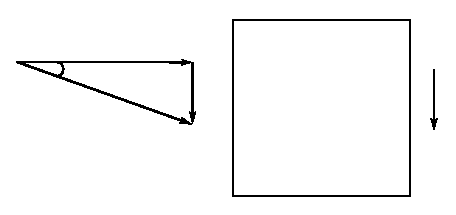
\includegraphics[width=0.5\unitlength]{../FnP/gnuplot/setup-1.eps}}         
      
      
   
 	\put(0.315,0.93){$U$}
 	\put(0.3,0.84){$U_i$}
    \put(0.42,0.88){$\dot{y}$}
    \put(0.28,0.895){ $\theta$}
    \put(0.7,0.87){\small $(+)$}
      	

 	
 	 

     

  \end{picture}

 \caption{Induced angle of attack on the square prism due to the resultant of free-stream velocity of the fluid and transverse velocity of the body.}
    \label{fig:setup_1}
\end{figure}

In the QSS model, it is assumed that the force on the body at a given instantaneous incident angle $\theta$ (defined in figure \ref{fig:setup_1}) is the same as the mean force on a static body at the same incident angle, or angle of attack. The instantaneous value of $C_y$ is therefore determined by an interpolating polynomial based on the lift data for flow over a stationary body at various $\theta$. Using the relationship between $\theta$ and the instantaneous transverse velocity of the body $\dot{y}$ shown in figure \ref{fig:setup_1}, $C_y$ can be written as a function of $\dot{y}$. The order of the interpolation polynomial used to define this function has varied from study to study. For  example a $7^{th}$ order polynomial was used in \cite{Parkinson1964} and $3^{rd}$ order polynomial was used in \cite{Barrero-Gil2009}. \cite{Ng2005} concluded that using a $7^{th}$ order polynomial is sufficient and a polynomial higher than that of $7^{th}$ order doesn't provides a significantly better result. Thus a $7 ^{th}$ order interpolating polynomial is used in this present study. As a result, $C_y(\theta)$ (noting that theta is proportional to $\dot{y}/U$) is defined as
\begin{equation}
\label{cy ploynomial}
C_y(\theta)=a_1\left(\frac{\dot{y}}{U}\right)+a_3\left(\frac{\dot{y}}{U}\right)^3+a_5\left(\frac{\dot{y}}{U}\right)^5+a_7\left(\frac{\dot{y}}{U}\right)^7.
\end{equation}

%\begin{equation}
%\label{modified_equation_of_motion}
%\ddot{y}+c^*\dot{y}+k^*y=\frac{1}{2}\rho U^2A
%\end{equation}

 It is expected that vortex shedding will be well correlated along the span and provide significant forcing at low \reynoldsnumber. \citet{Joly2012} introduced  an additional sinusoidal forcing function to the hydrodynamic forcing to model this. This enables the model to provide accurate predictions even at low mass ratios where galloping excitation is suppressed or not present. In this study, the forcing due to vortex shedding in low \reynoldsnumber\ cases is incorporated using a sinusoidal forcing function $F_0\sin{\omega_{s}t}$ added to the right-hand side of equation \ref{equationofmotion}. Here, $\omega_{s}$ and $F_0$ represent the angular vortex shedding frequency and the maximum force due to shedding respectively. Thus, the final equation for the modified QSS model is

\begin{equation}
\label{final_equation_motion}
m\ddot{y}{+}c\dot{y}{+}ky{=}\frac{1}{2}\rho U^2 \mathcal  {A} \Bigg(a_1\left(\frac{\dot{y}}{U}\right){+}a_3\left(\frac{\dot{y}}{U}\right)^3{+}a_5\left(\frac{\dot{y}}{U}\right)^5{+}a_7\left(\frac{\dot{y}}{U}\right)^7 \Bigg){+} F_0\sin{(\omega_s t)}.
\end{equation}

This equation can be solved using standard time integration methods. In this study the fourth-order Runge-Kutta scheme built in to the MATLAB routine `ode45' was generally used to obtain the solutions. Some low mass ratio cases used a solver modified for stiff problems, built into the `ode15s' routine in MATLAB.

\subsection{Calculation of average power}

 The dissipated power due to the mechanical damping represents the ideal potential amount of harvested power output. Therefore, the mean power output can be given by
\begin{equation}
\label{power}
P_{mean}=\frac{1}{T}\int_{0}^{T}(c\dot{y})\dot{y} dt,
\end{equation}
where $T$ is the period of integration and $c$ is the mechanical damping constant. 

It should be noted that this quantity is equal to the work done on the body by the fluid, defined as
\begin{equation}
\label{power_alt}
P_{mean}=\frac{1}{T}\int_{0}^{T}F_y\dot{y} dt,
\end{equation}
where $F_y$ is the transverse (lift) force.

These two definitions show two important interpretions of the power with respect to any energy production device. The first shows that power will be high for situations where the damping coefficient is high, and the transverse velocity is consistently high. The second shows that power will be high for situations where the transverse force and the body velocity are in phase.
 
 \begin{figure}

  \setlength{\unitlength}{\textwidth}
  \begin{picture}(1,0.25)(0,0.8)
  
    % % %90
      \put(0.025,0.81){\includegraphics[width=0.5\unitlength]{../FnP/gnuplot/lift_curve_165.eps}}
      \put(0.495,0.81){\includegraphics[width=0.5\unitlength]{../FnP/gnuplot/lift_curve_park.eps}}
 	\put(0.02,0.93){ \large $C_y$} 	
% 	\put(0.56,1.02){ $\theta$}
 	
        \put(0.25,0.8){ $\theta$} 	
        \put(0.75,0.8){ $\theta$}
        
        \put(0.105,1.01){(a)}
        \put(0.565,1.01){(b)}
      \end{picture}

  \caption{Lift coefficient, $C_y$, as a function of incidence angle $\theta$, for a static square cross section. (a) Data from simulations at $Re=165$  (b) data from \cite{Parkinson1964} at $Re=22300$. Points ($\bullet$) are measurements from the simulations. The solid lines in both plots are 7th-order interpolating polynomial used to predict the fluid forcing for the QSS model.}
    \label{fig:lift_curves}
\end{figure}

 \begin{table}[ht]

\begin{center}
\setlength{\unitlength}{\textwidth}

\begin{tabular}{c c c c c} % centered columns (4 columns)
\hline\hline %inserts double horizontal lines
\\[0.2ex]
Case & $a_1$ & $a_3$ & $a_5$ & $a_7$ \\ [0.8ex] % inserts table 
%heading
\hline 
\\[0.8ex]% inserts single horizontal line
Re=165 & 1.3 & 125.3 & 1825.73 & 8765.3 \\[0.8ex] % inserting body of the table
Re=22300 & 2.69 & 168 & 1670 & 59900 \\ [1ex] % [1ex] adds vertical space
\hline %inserts single line
\end{tabular}

\caption{Coefficient values used in the 7th order interpolation polynomial for high ($Re=22300$) and low ($Re=165$) Reynolds numbers. These data are used as input data to calculate the RHS of Eq.\ref{final_equation_motion} throughout this study.}
 
\label{table:nonlin} % is used to refer this table in the text
\end{center}
\end{table}


 
\subsection{Parameters used} 
 
For the low \reynoldsnumber\ tests, $\reynoldsnumber=165$ was maintained as it was pointed out by \citet{Sheard2009} and \citet{Tong2008} that the three-dimensional transition for a square cylinder occurs at approximately \reynoldsnumber=160. $F_0$ was kept at $0.4937$ which was obtained by scaling the value used by \citet{Joly2012} with the amplitude ratios of the lift forces obtained at the different Reynolds numbers. 

The angular vortex shedding frequency $\omega_s$, was set to $0.98$ which was obtained by performing a power spectral analysis of the stationary data at $0^\circ$. Stationary $C_y$ data were obtained at different angles of attack ranging from $0^\circ$ to $16^\circ$. The average power was obtained by using equation \ref{power}, and the averaging was done over no less than 20 galloping periods. Predictions of power output at $\reynoldsnumber=22300$ were obtained using the coefficients for curve fitting $C_y$ (Table (\ref{table:cy-coefficients})) from \citet{Parkinson1964}, in order to provide a comparison between high and low Reynolds numbers. The mass ratio $m^*$ was kept at 1163 for $\reynoldsnumber=22300$ (Similar to \citet{Parkinson1964}) and $m^*=20$ for \reynoldsnumber=165. These parameters were used throughout this study unless otherwise specified. 

The stationary data and the fluid-structure interaction (FSI) data were obtained using a high-order spectral element routine to simulate the two-dimensional laminar flow.  Simulations involving fluid structure interaction (FSI) were used to provide additional validation of the QSS model. The inlet was placed $20D$ while the outlet situated $60D$ away from the centroid of the body. The side boundaries were placed $20D$ away from the centroid of the body where $D$ was kept as unity throughout this study. The Navier--Stokes equations were solved in an accelerated frame of reference attached to the moving body along with the body equation of motion given in equation \ref{equationofmotion}. A three-step time splitting scheme together with high-order Lagrangian polynomials were used to obtain the solution. The details of the method can be found in \citet{Thompson2006,Thompson1996a}. This code has been very well validated in a variety of fluid-structure interaction problems \citep{Leontini2007a,Griffith2011,Leontini2011,Leontini2013}.
 
The computational domain consists of 690 quadrilateral macro elements where the majority of the elements were concentrated near the square section. A freestream condition was given to the inlet, top and bottom boundaries and the normal velocity gradient was set to zero at the outlet. A convergence study was performed by changing the order of the polynomial ($p$-refinement) at $U^*=40$ and $\reynoldsnumber=165$. A $9^{th}$ order polynomial together with a time step of $\Delta tU/D=0.001$ was sufficient to ensure an accuracy of $2\%$ with regards to amplitude of oscillation.








%\section{Results}

\subsection{Stationary data}

The stationary $C_y$ data obtained using flow simulations (Fig.\ref{cy ploynomial}(a)) have a good agreement with data presented in \cite{Joly2012}. In comparison with the 7th order polynomial curve at \reynoldsnumber=22300 (Fig.\ref{cy ploynomial}(b)),  several differences could be observed. The peak value of $C_y$ is  significantly low at \reynoldsnumber=165 ($C_y=0.05$ at $4^0$) in comparison with \reynoldsnumber=22300 ($C_y=0.57$ at $13^0$) . The inflection point present at \reynoldsnumber=22300 could not be observed at \reynoldsnumber=165. This agrees with the findings of \cite{Luo2003}. It was concluded by \cite{Luo2003} that hysteresis occur due to the inflection point found in the $C_y$ curve. Therefore hysteresis is not expected at \reynoldsnumber=165. The range of the incident flow angles where $C_y$ remain positive is narrow at \reynoldsnumber=165 ($0^0 <\theta \leq$ $6^0$) compared to \reynoldsnumber=22300 ($0^0 <\theta \leq 15^0$). This feature is what sustains galloping and power is transferred from the fluid to the supporting structure within this range of incident angles because fluid forces are acting in the direction of travel of the oscillating cylinder. Incident angles beyond this range actually suppresses the galloping and power goes in the opposite direction. Therefore due to the overall smaller $C_y$ and narrow range of angles where $C_y$ is positive for \reynoldsnumber=165 compared to \reynoldsnumber=22300 leads one to expect a significant reduction in power at\reynoldsnumber=165 compared to \reynoldsnumber=2230.

  

\begin{figure}
  \setlength{\unitlength}{\textwidth}

  \begin{picture}(1,0.72)
%(0,0.35)
    
    % % %Parkinson Data 
    \put(0.025,0.48){\includegraphics[width=0.5\unitlength]{../FnP/gnuplot/displacement_amp_re_parkinson_1.eps}}
    \put(0.025,0.25){\includegraphics[width=0.5\unitlength]{../FnP/gnuplot/velocity_amp_re_parkinson.eps}}
    \put(0.025,0.02){\includegraphics[width=0.5\unitlength]{../FnP/gnuplot/mean_power_re_parkinson.eps}}
    
    % Re 165 Data 
    \put(0.495,0.48){\includegraphics[width=0.5\unitlength]{../FnP/gnuplot/displacement_amp_re165.eps}}
    \put(0.495,0.25){\includegraphics[width=0.5\unitlength]{../FnP/gnuplot/velocity_amp_re165.eps}}
    \put(0.495,0.02){\includegraphics[width=0.5\unitlength]{../FnP/gnuplot/mean_power_re_165.eps}}
   
%    \put(0.25,0.93){\ustar}
%    \put(0.8,0.93){\ustar}
%    \put(0.25,0.63){\ustar}
%   \put(0.8,0.63){\ustar}
    \put(0.25,0.0){\ustar}
    \put(0.75,0.0){\ustar}
    
    \put(0.00,0.6){$\displaystyle\frac{A}{D}$}
%    \put(0.52,1.075){$\frac{A}{D}$}
    \put(0.00,0.4){$\displaystyle\frac{V}{D}$}
%    \put(0.52,0.83){$\frac{V}{D}$}
    \put(-0.025,0.15){$\displaystyle\frac{P_{m}}{\rho \mathcal{A}U^3 }$}
%    \put(0.5,0.54){$\frac{P_{m}}{\rho \mathcal{A}U^3 }$}
    
    \put(0.085,0.685){\small(a)}
    \put(0.555,0.685){\small(b)}
    \put(0.085,0.455){\small(c)}
    \put(0.555,0.455){\small(d)}
    \put(0.085,0.225){\small(e)}
    \put(0.555,0.225){\small(f)}   
  \end{picture}

%  \vspace{-4cm}
  \caption{Velocity amplitude, displacement amplitude and mean power  as functions of $U^*$. Data presented in (a), (c) and (e) were calculated using input data at $Re=22300$ and $m^*=1163$ obtained by \cite{Parkinson1964} at three different damping ratios: $\zeta=0.0125$ (\ding{83}), $\zeta=0.015$ (\ding{116}) and $\zeta=0.0175$ (\ding{108}). Data presented in (b),(d) and (f) were obtained using input data at $Re=165$ and $m^*=20$ at three different damping ratios: $\zeta=0.075$ ($\times$), $\zeta=0.1$ (\ding{117}) and $\zeta=0.15$ (+). The multiple branches for the higher Re are due to the hysteresis between two solutions.}
  
\label{fig:uncollapsed_data}
\end{figure}




\subsection{Displacement,velocity and power output as a function of reduced velocity}


 The quasi-steady analysis data reveals that the displacement amplitude tend to grow with increasing $U^*$ (Fig.\ref{fig:uncollapsed_data} (a) and (b)). The onset of galloping is delayed with increasing $\zeta$ for both high and low Reynolds numbers. This echo the findings of previous studies by \cite{Parkinson1964} and \cite{Barrero-Gil2010a}. Hysteresis could be observed for the case with a higher Reynolds number. This was achieved by manipulating the initial conditions (initial displacement) of the system. The upper branch was obtained by giving an initial displacement which was higher than the expected amplitude while the lower branch was obtained by providing a lower initial displacement than the expected amplitude. Although a third state could be achieved theoretically, it was not possible to achieve numerically. This was also observed by \cite{Vio2007}.   

 
 \subsubsection*{Power vs $U^*$}
 
 The mean power grows, peaks and then reduces as $U^*$ is increased (Fig.\ref{fig:uncollapsed_data} (e) and (f)) for each value of $\zeta$. The value of  \ustar at which the peak power occur increases with $\zeta$. However, the magnitude of the peaks remain constant for all the values of $\zeta$.  \cite{Barrero-Gil2010a} also showed a similar trend. The higher Reynolds number case clearly showed hysteresis in the power data. The range of hysteresis tend to increase with increasing $\zeta$. It could be observed that unlike VIV the  system has no preferred frequency. Although the onset of galloping and the point where peak power occur at different $U^*$ when the damping ratio is changed, the peak power remains constant regardless of $U^*$.
 
 \subsection{Galloping response and natural frequency}
 
 Now the oscillator equation Eq.\eqref{final_equation_motion} is considered from a power perspective. The shedding forces can be neglected because the net effect is negligible as system oscillates at natural frequency which is far from shedding frequency, for the cases that exhibit galloping. It is obvious that the forcing term on LHS of the equation is only dependent on transverse velocity($\dot{y}$) which is essentially the input power of the system. On the RHS, the mechanical damping or system damping is the only term that takes out power at any instant. This could be expressed as the product of the damping force and the velocity ($P_d$). The inertia and the stiffness terms governs the frequency of the system but the forces associated by those terms are conservative forces (i.e there is zero net energy in or out of the system when averaged over a period). Therefore the system is governed by the transverse velocity rather than the natural frequency.
 

 Using $U^*$ and $\zeta$ assumes that the system has a preferred frequency because the scale with the natural frequency of the system. The effect of fixing $\zeta$ and increasing $U^*$ actually decreases the damping constant for a fixed free-stream velocity. ($U^*=\frac{U}{f \times D}$, $\zeta= \frac{c}{2 m \omega_n}$ ). Both these effects leads to the multiple lines that are horizontally transpose when $\zeta$ is increased (Fig.\ref{fig:uncollapsed_data} (e) and (f)). Therefore the effect of $\zeta$ essentially scales up the damping coefficient for a fixed $U^*$.
 
 The data presented in Fig.\ref{fig:uncollapsed_data} for various damping ratios, $\zeta$, can be collapsed into a single line for a for a particular force characteristic curve (i.e $C_y$ vs $\theta$ curve). These collapsed curves were  obtained for the velocity amplitude  and power by plotting as functions of as a function of  the non dimensionalised  damping constant $\frac{c}{\rho\mathcal{A}U}$ 
(Fig \ref{fig:collpased_data} (a),(b),(c) and (d)).  This further emphasizes that the galloping system is not frequency dependent. It is possible to obtain a different similar power output at different values of \ustar when the damping constant, $\frac{c}{\rho\mathcal{A}U}$, is kept fixed. An example of this case, as shown in Fig.\ref{fig:time_hostory_velocity_same_power}, clearly show that this is a result of similar velocity amplitudes between cases if one were to disregard the high frequencies due to shedding. As mentioned earlier, it is the transverse velocity that determines the energy provided by the fluid forcing and the mechanical damping.

\begin{figure}
  \setlength{\unitlength}{\textwidth}

        \begin{picture}(1,0.74)

      % % % Parkinson Data 
      \put(0.025,0.5){\includegraphics[width=0.5\unitlength]{../FnP/gnuplot/displacement_amp_collapsed_parkinson.eps}}
      \put(0.025,0.27){\includegraphics[width=0.5\unitlength]{../FnP/gnuplot/velocity_amp_collapsed_parkinson.eps}}
      \put(0.495,0.27){\includegraphics[width=0.5\unitlength]{../FnP/gnuplot/velocity_amp_collapsed_re165.eps}}
      
      \put(0.025,0.02){\includegraphics[width=0.5\unitlength]{../FnP/gnuplot/mean_power_collapsed_parkinson.eps}}
      \put(0.495,0.02){\includegraphics[width=0.5\unitlength]{../FnP/gnuplot/mean_power_collapsed_re_165.eps}}
      \put(0.495,0.5){\includegraphics[width=0.5\unitlength]{../FnP/gnuplot/displacement_amp_collpased_re165.eps}}
      
      \put(0.23,0.00){ $\displaystyle\frac{c}{\rho\mathcal{A}U}$}
      \put(0.73,0.00){ $\displaystyle\frac{c}{\rho\mathcal{A}U}$}
      
      \put(0.01,0.405){$\displaystyle\frac{V}{D}$}\
       \put(0.01,0.63){$\displaystyle\frac{A}{D}$}
      
      \put(-0.02,0.13){$\displaystyle\frac{P_{m}}{\rho \mathcal{A}U^3 }$}
      
      \put(0.46,0.709){\small(a)}
      \put(0.93,0.709){\small(b)}
      \put(0.46,0.475){\small(c)}
      \put(0.93,0.475){\small(d)}
      \put(0.46,0.225){\small(e)}
      \put(0.935,0.225){\small(f)}
      
    \end{picture}

  \caption{Displacement amplitude, velocity amplitude and mean power as functions of the damping factor. Data presented in (a),(c) and (e)  were calculated using input data at $Re=22300$ obtained by \cite{Parkinson1964} at three different damping ratios: $\zeta=0.0125$ (\ding{83}), $\zeta=0.015$ (\ding{116}) and $\zeta=0.0175$ (\ding{108}). Data presented in (b), (d) and (f)  were obtained using input data at $Re=165$ at three different damping ratios: $\zeta=0.075$ ($\times$), $\zeta=0.1$ (\ding{117}) and $\zeta=0.15$ (+). The collapsed data implies that there is no frequency selection and the tuning parameter of the mechanical side of the system is the damping constant to obtain an optimum power output.}
    \label{fig:collpased_data}
\end{figure}

 %vspace{10cm}

 
\begin{figure}
  \setlength{\unitlength}{\textwidth}
  \begin{picture}(1,0.3)(0,0.8)
    % % %90
    \put(0.025,0.83){\includegraphics[width=0.5\unitlength]{../FnP/gnuplot/vel_time_history_60_0.075.eps}}
    \put(0.495,0.83){\includegraphics[width=0.5\unitlength]{../FnP/gnuplot/vel_time_history_165_0.175.eps}}
    
    \put(0.03,0.95){ $\frac{V}{D}$} 	
    % \put(0.56,1.02){ $\frac{V}{D}$}
 	
    \put(0.25,0.805){ $\frac{tU}{D}$} 	
    \put(0.73,0.805){ $\frac{tU}{D}$}

    \put(0.095,1.03){(a)}
    \put(0.565,1.03){(b)}

  \end{picture}

  \caption{Time histories of velocity at two different $\zeta$ and $U^*$ which produce the same mean power ($1.2\times10^{-3}$). Data presented in (a) are at $\ustar=60$, $\zeta=0.075$ and (b) are at $\ustar=165$, $\zeta=0.175$. Both data sets were obtained using Quasi-steady state assumption using input $C_y$ parameters at $Re=165$. Shedding is evident in both signals as a high frequency fluctuation but the amplitude of the slower fluctuations remains constant in both cases.}
    \label{fig:time_hostory_velocity_same_power}
\end{figure}

 


 
 Power could be expressed as the product of force and velocity. Therefore the transferred power form fluid-to-body could be expressed as $P_t=F_y\dot{y}$. Similarly the dissipated power due to the mechanical damping could be expressed as $P_d=(c\dot{y})\dot{y}$. The time average of these two quantities should be equal due to energy conservation, provided that the mechanical friction is neglected . Analysing the  time histories of $P_t $ and $P_d$ at key regions (Fig.\ref{fig:regions_1}) on the mean power vs $U^*$ provides a detailed explanation for the variation of the output power when the reduced velocity is increased. The key regions consists of region 1 where the $P_{mean}$ increases with \ustar, region 2 where $P_{mean}$ becomes maximum and region 3 where $P_{mean}$ decreases with \ustar. It has been established earlier that the damping factor is a function of $U^*$. Therefore it could be derived that $U^*$ is inversely proportional to damping coefficient. Hence the damping coefficient reduces when you move from region 1 to 3. Fig \ref{fig:lift_curves} (a) shows that $C_y$ and therefore instantaneous force rises until $4^0$ where it peaks and then falls and at around $6^0$ becomes negative. Maximum amount of power could be transferred within the peak region. At the region where the instantaneous force becomes negative it will be opposing the velocity $\dot{y}$. Data at $\zeta=0.1$, $m^*=40$ and \reynoldsnumber=165 (Fig.\ref{fig:power_time_histories}) are analysed as and example.  

\begin{figure}[h!]
\centering
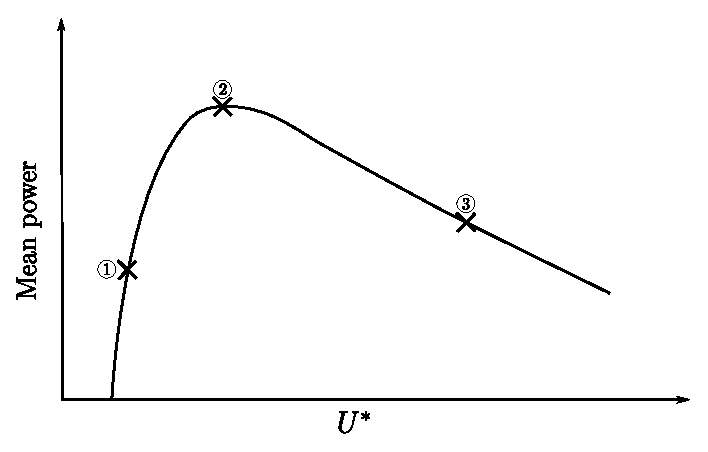
\includegraphics[width=0.5\textwidth]{../FnP/sketch_1}
\caption{ Three key regions taken into account to analyse the time histories of power in a typical mean power vs. $U^*$ curve at $Re=165$. In region 1, high damping suppresses oscillation, hence the power output is low. In region 2, the damping is close to the optimum for power transfer. In region 3, the low damping means little energy is extracted from the fluid.}
\label{fig:regions_1}
\end{figure}

 
 
 
 At region 1 where $U^*=90$ the damping constant is high and a clear sinusoidal signal could be observed for both $P_d$ and $P_t$ in Fig.\ref{fig:power_time_histories} (a). Fig.\ref{fig:power_time_histories} (d) and (g) shows that $\theta$ is in line or in phase with $F_y$.  The velocity amplitude in this case is small and the equivalent incident angle within the range where the hydrodynamic force increases with the incident angle (i.e. $0<\theta \leq < 4^0$ in Fig.\ref{fig:lift_curves} (a)) Hence both $P_d$ and $P_t$ becomes sinusoidal. In this case, power output is limited by the low fluid forces present at low incident angles. In other words damping is significantly high and extracts a lot of power that the velocity amplitude could not grow where the forcing  is significant to produce high level of power.   
 
 
  At region 3 ($U^*= 400$) `$c$' is low in comparison with region 1 and 2 which leads to a low mean power output. Fig.\ref{fig:power_time_histories} (c) shows that $P_t$ becomes negative over some portion of the cycle. This is because $\theta$  passes the point where both $\theta$ and $C_y$ (therefore $F_y$) are positive. The high velocity amplitude leads to the equivalent incident angle $\theta$, in this case to exceed the range where $C_y$ is positive (i.e. $0<\theta<6^0$ in Fig.\ref{cy ploynomial} (a)). In this portion of the cycle the hydrodynamic force actually opposes the direction of travel and power is transferred from the structure to the fluid during those times. From and energy perspective, the mechanical damping is not sufficient to remover the energy transferred from the fluid to the structure during other times of the cycle because $\frac{c}{\rho\mathcal{A}U}$ is substantially low. Therefore this excess energy is transferred back to the fluid as depicted by the negative region of $P_d$ in Fig.\ref{fig:power_time_histories} (c) 
 

At region 2 ($U^*=165$). $P_t$ is not a pure sinusoidal signal. However, the  signal remains periodic. From the time history graph of $P_t$, two `peaks' are present in a single half cycle (Fig \ref{fig:power_time_histories} (b)). In this case, the velocity amplitude actually exceeds the equivalent incident angle where the hydrodynamic forces peaks (i.e. $\theta=4^0$ in \ref{cy ploynomial} (a)). The dips in $P_d$ between the two peaks approximately correspond to the time where the transverse velocity is higher than 0.07 and $F_y$ is decreasing with increasing transverse velocity. The mean power output is at its maximum. This is due to the fact that this region is a best compromise between region 1 and 3. The damping is substantially high to obtain a high power output while not too high to hinder the induced angle of attack entering the region where the forcing is high. 


 
  
\begin{figure}

  \setlength{\unitlength}{\textwidth}
%  \fbox{
  \begin{picture}(1,0.58)(0,0.35)
    % % % 90
    \put(0.03,0.76){\includegraphics[width=0.35\unitlength]{../FnP/gnuplot/power_time_history_90.eps}}
    \put(0.03,.58){\includegraphics[width=0.35\unitlength]{../FnP/gnuplot/f_y_history_90.eps}}
    \put(0.03,0.4){\includegraphics[width=0.35\unitlength]{../FnP/gnuplot/theta_time_history_90.eps}}
    
    % % 165
    \put(0.36,0.76){\includegraphics[width=0.35\unitlength]{../FnP/gnuplot/power_time_history_165.eps}}
    \put(0.36,.58){\includegraphics[width=0.35\unitlength]{../FnP/gnuplot/f_y_history_165.eps}}
    \put(0.36,0.4){\includegraphics[width=0.35\unitlength]{../FnP/gnuplot/theta_time_history_165.eps}}
    
    \put(0.68,0.76){\includegraphics[width=0.35\unitlength]{../FnP/gnuplot/power_time_history_400.eps}}
    \put(0.68,.58){\includegraphics[width=0.35\unitlength]{../FnP/gnuplot/f_y_history_400.eps}}
    \put(0.68,0.4){\includegraphics[width=0.35\unitlength]{../FnP/gnuplot/theta_time_history_400.eps}}
    
    \put(0.55,0.36){$\displaystyle{\frac{tU}{D}}$}
    \put(0.2,0.36){$\displaystyle{\frac{tU}{D}}$}
    \put(0.85,0.36){$\displaystyle{\frac{tU}{D}}$}
    
    \put(0.0,0.87){$\frac{P}{\rho \mathcal{A}U^3}$}
    \put(0.01,0.66){$F_y$}
    \put(0.01,0.49){$\theta$}
    
    \put(0.08,0.76){(a)}
    \put(0.08,0.58){(d)}
    \put(0.08,0.38){(g)}
    
    \put(0.4,0.76){(b)}
    \put(0.4,0.58){(e)}
    \put(0.4,0.38){(h)}
    
    \put(0.72,0.76){(c)}
    \put(0.72,0.58){(f)}
    \put(0.72,0.38){(i)}
  \end{picture}
%}
  \caption{Time histories of $P_t$, $P_d$, $F_y$ and $\theta$ at $\ustar=90$, $165$ and $400$. Data was obtained at $\zeta=0.1$, $m^*=40$ and \reynoldsnumber=165. The time histories of $P_t$ ( \solidrule[4mm]\hspace{1mm}) and $P_d$ (\protect\dashedrule) are presented for: (a) $\ustar = 90$; (b) $\ustar = 165$; (c) $\ustar = 400$. Time histories of the instantaneous force $F_y$ for: (d) $\ustar = 90$; (e $\ustar = 165$; (f) $\ustar = 400$. Time histories of the instantaneous angle $\theta$ for: (g) $\ustar = 90$; (h) $\ustar = 165$; (i) $\ustar = 400$.}
  \label{fig:power_time_histories}
\end{figure}







\subsection{Effect of $m^*$}

 \begin{figure}

\setlength{\unitlength}{\textwidth}
\fbox{
  \begin{picture}(1,0.32)
    
       \put(0.07,0.03){\includegraphics[width=0.3\unitlength]{../FnP/gnuplot/mean_power_collapsed_mstar.eps}}
       \put(0.36,0.03){\includegraphics[width=0.3\unitlength]{../FnP/gnuplot/mean_power_collapsed_noshed_mstar.eps}}
       \put(0.65,0.03){\includegraphics[width=0.3\unitlength]{../FnP/gnuplot/fsi_power.eps}}
        
        \put(0.03,0.17){\large $\frac{P_{m}}{\rho \mathcal{A}U^3}$}
              
        \put(0.2,0.0){$\frac{c}{\rho\mathcal{A}U}$} 	
        \put(0.49,0.0){$\frac{c}{\rho\mathcal{A}U}$}
        \put(0.78,0.0){$\frac{c}{\rho\mathcal{A}U}$}
    
        \put(0.133,0.21){\small(a)}
        \put(0.42,0.21){\small(b)}
        \put(0.715,0.21){\small(c)}
    
 

     

  \end{picture}
  }

  \caption{Mean power as a function of damping factor. Data are presented at $m^*=10$ (\ding{108}), $m^*=20$ (\ding{83}), $m^*=40$ (\ding{115}), $m^*=60$ (+) at Re 165 and $\zeta=0.1$. A reduction of maximum mean power can be observed when $m^*<40$. For $m^*>40$, the maximum power is essentially independent of $m^*$.}
    \label{fig:m_star_collapsed}
\end{figure}



Mean power as a function of damping factor at Re
 \begin{figure}
  \setlength{\unitlength}{\textwidth}

        \begin{picture}(1,0.3)(0.0,0.45)

      % % % Parkinson Data 
      \put(0.025,0.5){\includegraphics[width=0.5\unitlength]{../FnP/gnuplot/mean_power_collapsed_mstar_175.eps}}      \put(0.495,0.5){\includegraphics[width=0.5\unitlength]{../FnP/gnuplot/mean_power_collapsed_parkinson_10.eps}}
      
      \put(0.23,0.48){ $\displaystyle\frac{c}{\rho\mathcal{A}U}$}
      \put(0.73,0.48){ $\displaystyle\frac{c}{\rho\mathcal{A}U}$}
          
      \put(0.0,0.63){\large$\frac{P_{m}}{\rho \mathcal{A}U^3 }$}
      
      \put(0.085,0.709){\small(a)}
      \put(0.555,0.709){\small(b)}
     
      
    \end{picture}
  \caption{Mean power as a function of damping factor. Data presented in both (a) and (b) were calculated using input data at \reynoldsnumber=22300 \cite{Parkinson1964} where (a) shows mean power data at six different mass ratios: $m^*=1164$ (\ding{83}), $m^*=100$ (\ding{116}), $m^*=50$ (\ding{108}), $m^*=10$ (+), $m^*=5$ (\ding{110}) and $m^*=1$ ($\times)$ at \ustar=175. Data presented in (b) shows mean power data at three different reduced velocities: \ustar=75 (\ding{108}), \ustar=175 (\ding{116}) and \ustar=375 (\ding{83}) at $m^*=10$. The maximum mean power tend to increase with decreasing $m^*$ as well as increasing \ustar at low $m^*$.}  
    
    \label{fig:mstarcollapsed_parkinson}
\end{figure}

\ %vspace{10cm}


The maximum mean power at different $m^*$ (Fig.\ref{fig:m_star_collapsed}(a)) was constant for $m^*>30$ in the low \reynoldsnumber\ case. However, at $m^* \leq 30$, the power output reduces with reducing $m^*$ across the parameter range. However, when the sinusoidal forcing function in Eq.\ref{equationofmotion} which cater for the vortex shedding was disregarded, the reduction in power could not be observed Fig.\ref{fig:m_star_collapsed}(b). The suppression of galloping response at low $m^*$ due to the presence of vortex shedding has previously been observed by \cite{Joly2012}. This is a non-linear interaction between the forcing that drives the galloping excitation and the forcing as a result of vortex shedding. The forcing associated with vortex  shedding is significantly larger and at a higher frequency than the forcing that drives galloping. Systems with low $m^*$ do not have enough inertia to fully sustain the galloping excitation over the longer period.

At \reynoldsnumber=22300 power output started to increase for cases with $m^*<50$. The overall mean power tend to increase  as the $m^*$ was decreased when $U^*$ was kept constant (Fig\ref{fig:mstarcollapsed_parkinson} (a)). The same effect was observed when $U^*$ was increased keeping $m^*$ constant (\ref{fig:mstarcollapsed_parkinson} (b)). It should be noted that the influence of $U^*$ was observed only for low mass ratios.  The velocity time traces of example cases of both scenarios presented in Fig.\ref{time_hostory_mstar_mass} and \ref{time_history_mstar_ustar} shows that essentially the same phenomenon occurring in both cases whereby the velocity signal tend to shift from a sinusoidal signal towards a square wave. The corresponding displacement signal tend to become more like a triangular wave. When the inertia of the system reduces, the body can accelerate faster thus attaining higher velocities more rapidly and spend a higher proportion of the period at a high velocity. Higher velocities are favourable because they result in higher instantaneous hydrodynamic forcing and power output from mechanical damping. However, the velocity is limited by the characteristic of the hydrodynamics forcing which reaches a maximum and then decreases past an incident angle of of $6 ^\circ$ which correspond to a transverse velocity of $\frac{\dot{y}}{U}=0.1$. Increasing $U^*$ effectively reduces the stiffness of the system and lengthen the period, thus again allowing a larger portion of the period to be at a high velocity which favours power output. For the case of fixing $U^*$ and decreasing $m^*$ in (Fig\ref{fig:mstarcollapsed_parkinson} (a)), the lengthening of the period is associated with the added mass which is kept constant at ??? being more dominant on the overall mass of the system when m* is reduced.

  




\begin{figure}

   \setlength{\unitlength}{\textwidth}

   \begin{picture}(1,0.399)(0.01,0.77)
     % % % 90
     \put(0.03,1){\includegraphics[width=0.35\unitlength]{../FnP/gnuplot/vel_time_history_75.eps}}   
     \put(0.36,1){\includegraphics[width=0.35\unitlength]{../FnP/gnuplot/vel_time_history_175.eps}}
     \put(0.68,1){\includegraphics[width=0.35\unitlength]{../FnP/gnuplot/vel_time_history_375.eps}}
         
     \put(0.03,0.82){\includegraphics[width=0.35\unitlength]{../FnP/gnuplot/dis_time_history_75.eps}}   
     \put(0.36,0.82){\includegraphics[width=0.35\unitlength]{../FnP/gnuplot/dis_time_history_175.eps}}
     \put(0.68,0.82){\includegraphics[width=0.35\unitlength]{../FnP/gnuplot/dis_time_history_375.eps}}
     
 
     
     \put(0.55,0.79){$\displaystyle{\frac{tU}{D}}$}
     \put(0.2,0.79){$\displaystyle{\frac{tU}{D}}$}
     \put(0.85,0.79){$\displaystyle{\frac{tU}{D}}$}
     
      \put(0.02,1.07){$\displaystyle\frac{V}{D}$}
     \put(0.02,0.9){$\displaystyle\frac{A}{D}$}
 
     
     \put(0.08,0.9997){(a)}    
     \put(0.4,0.9997){(b)}    
     \put(0.72,0.9997){(c)}
     \put(0.08,0.8){(d)}    
     \put(0.4,0.8){(e)}    
     \put(0.72,0.8){(f)}
     
    
   \end{picture}

   \caption{Time histories of displacement and velocity at \reynoldsnumber=22300, \ustar=175 and $\massdamp=9.3\times10^{-1}$. The velocity time histories are presented for: (a) $m^*=1164$; (b) $m^*=10$; (c) $m^*=5$. The time histories of displacement are presented for: (d) $m^*=1164$; (e) $m^*=10$; (f) $m^*=5$. As the mass ratio decreases the velocity signal tend to transform from a sinusoidal towards a square signal and the displacement signal tend to move towards a triangular signal due to reduction in inertia.}
  
  \label{time_hostory_mstar_mass}
\end{figure}






\begin{figure}

  \setlength{\unitlength}{\textwidth}
  
 \begin{picture}(1,0.399)(0.01,0.77)
     % % % 90
     \put(0.03,1){\includegraphics[width=0.35\unitlength]{../FnP/gnuplot/vel_time_history_1164.eps}}   
     \put(0.36,1){\includegraphics[width=0.35\unitlength]{../FnP/gnuplot/vel_time_history_10.eps}}
     \put(0.68,1){\includegraphics[width=0.35\unitlength]{../FnP/gnuplot/vel_time_history_5.eps}}
         
     \put(0.03,0.82){\includegraphics[width=0.35\unitlength]{../FnP/gnuplot/dis_time_history_1164.eps}}   
     \put(0.36,0.82){\includegraphics[width=0.35\unitlength]{../FnP/gnuplot/dis_time_history_10.eps}}
     \put(0.68,0.82){\includegraphics[width=0.35\unitlength]{../FnP/gnuplot/dis_time_history_5.eps}}
     
 
     
     \put(0.55,0.79){$\displaystyle{\frac{tU}{D}}$}
     \put(0.2,0.79){$\displaystyle{\frac{tU}{D}}$}
     \put(0.85,0.79){$\displaystyle{\frac{tU}{D}}$}
     
      \put(0.02,1.07){$\displaystyle\frac{V}{D}$}
     \put(0.02,0.9){$\displaystyle\frac{A}{D}$}
 
     
     \put(0.08,0.9997){(a)}    
     \put(0.4,0.9997){(b)}    
     \put(0.72,0.9997){(c)}
     \put(0.08,0.8){(d)}    
     \put(0.4,0.8){(e)}    
     \put(0.72,0.8){(f)}
     
    
   \end{picture}


   \caption{  Time histories of displacement and velocity at \reynoldsnumber=22300, $m^*=10$ and $\massdamp=9.3\times10^{-1}$. The velocity time histories are presented for: (a) \ustar=75; (b) \ustar=175 (c) \ustar=375. The time histories of displacement are presented for: (d) \ustar=75; (e) \ustar=175; (f) \ustar=375.   As the mass ratio decreases the velocity signal tend to transform from a sinusoidal towards a square signal and the displacement signal tend to move towards a triangular signal.}
  
 
  
  
  
  
  
  \label{time_history_mstar_ustar}
\end{figure}





\begin{figure}
  \setlength{\unitlength}{\textwidth}
  \begin{picture}(1,0.25)
    % % %90
    \put(0.02,0.03){\includegraphics[width=0.3\unitlength]{../FnP/gnuplot/fsi_displacement.eps}}
    \put(0.36,0.03){\includegraphics[width=0.3\unitlength]{../FnP/gnuplot/fsi_velocity.eps}}
    \put(0.72,0.03){\includegraphics[width=0.3\unitlength]{../FnP/gnuplot/fsi_power.eps}}
    
    \put(0.02,0.15){$\displaystyle\frac{A}{D}$}
    \put(0.35,0.15){$\displaystyle\frac{V}{D}$}
    \put(0.67,0.15){$\displaystyle\frac{P_{m}}{\rho \mathcal{A}U^3 }$}
    
    \put(0.18,0.01){\ustar} 	
    \put(0.51,0.01){\ustar}
    \put(0.87,0.01){\ustar}

    \put(0.092,0.21){\small(a)}
    \put(0.42,0.21){\small(b)}
    \put(0.78,0.21){\small(c)}

  \end{picture}  

  \caption{Comparison of data generated using the quasi-static theory (\ding{83}) and full DNS simulations (\ding{108}). (a) Displacement amplitude, (b) velocity amplitude and (c) mean power as functions of \ustar. Data were obtained at $Re=165$ and $\zeta=0.075$. An average difference of $34\%$ is observed for both displacement and velocity amplitude. However, the essential physics i.e the rise and fall of mean power, is captured by DNS simulations.}
    \label{fig:FSI_QSS_compare}
\end{figure}
 

\subsection{Comparison with FSI simulations}
 Similar trends were captured for both displacement and velocity amplitudes between QSS and FSI simulations (Fig. \ref{fig:FSI_QSS_compare}(a) and \ref{fig:FSI_QSS_compare}(b)). Quantitatively a large discrepancy (average of $30\%$) could be observed between QSS and FSI data. Therefore the power also becomes significantly low in FSI data (Fig.\ref{fig:FSI_QSS_compare} (c)). However, the FSI data (Fig.\ref{fig:FSI_QSS_compare} (c)) were able to produce the main the rise and the fall of mean power when $U^*$ was increased. The reasoning behind this fact is that galloping is weak at \reynoldsnumber$=165$  and therefore fluid damping has a significant effect. It was reported by \cite{Barrero-Gil2009} that galloping only starts to occur ar Re $\geq 159$. As power is function of $(\dot{y})^2$ the error between QSS and FSI power becomes significantly large.  
 

 

\section{Conclusion}

In this paper, the power transfer of a square body under aero elastic galloping is analysed by solving the quasi-steady state model equations through numerical integration. The power output of the system is not dependent on \ustar or natural frequency of the system, but dependent on the transverse velocity amplitude of the system. This is shown by the collapsed plots in terms of non-dimensionalised damping constant (using flow parameters). By analysing key regions of the power vs \ustar curve it could be concluded that in order to obtain an optimum power output, the damping constant ($\frac{c}{\rho\mathcal{A}U}$) should be high, but not excessive until it  to hinders the galloping from reaching induced angles of attack where the forcing is significant. The effect of mass ratio was could also be observed where at \reynoldsnumber=165. The mean power tend to decrease at $m^*<50$ which was found out to be an influence of vortex shedding. At \reynoldsnumber=22300 an opposite result could be observed where the mean power tend to increase with decreasing mass ratio as well as the mean power tend to increase with increasing $U^*$ at low mass ratios. The cause for this was found out to be the fact that when the mass ratio decreases, due to the lower inertia the velocity time trace tend to move from a sinusoidal signal towards a square signal where it sustains high velocities for longer periods of time which leads to a higher mean power output.






 

 
 
 

 
 


 % % % % % % % % % % % % % % % % % % % % % % % % % % % % % % % % % % % % % % % % %

 
 
 
 
 
 
 
 
 
 
  
 
 


%% The Appendices part is started with the command \appendix;
%% appendix sections are then done as normal sections
%% \appendix

%% \section{}
%% \label{}

%% References
%%
%% Following citation commands can be used in the body text:
%%
%%  \citet{key}  ==>>  Jones et al. (1990)
%%  \citep{key}  ==>>  (Jones et al., 1990)
%%
%% Multiple citations as normal:
%% \citep{key1,key2}         ==>> (Jones et al., 1990; Smith, 1989)
%%                            or  (Jones et al., 1990, 1991)
%%                            or  (Jones et al., 1990a,b)
%% \cite{key} is the equivalent of \citet{key} in author-year mode
%%
%% Full author lists may be forced with \citet* or \citep*, e.g.
%%   \citep*{key}            ==>> (Jones, Baker, and Williams, 1990)
%%
%% Optional notes as:
%%   \citep[chap. 2]{key}    ==>> (Jones et al., 1990, chap. 2)
%%   \citep[e.g.,][]{key}    ==>> (e.g., Jones et al., 1990)
%%   \citep[see][pg. 34]{key}==>> (see Jones et al., 1990, pg. 34)
%%  (Note: in standard LaTeX, only one note is allowed, after the ref.
%%   Here, one note is like the standard, two make pre- and post-notes.)
%%
%%   \citealt{key}          ==>> Jones et al. 1990
%%   \citealt*{key}         ==>> Jones, Baker, and Williams 1990
%%   \citealp{key}          ==>> Jones et al., 1990
%%   \citealp*{key}         ==>> Jones, Baker, and Williams, 1990
%%
%% Additional citation possibilities
%%   \citeauthor{key}       ==>> Jones et al.
%%   \citeauthor*{key}      ==>> Jones, Baker, and Williams
%%   \citeyear{key}         ==>> 1990
%%   \citeyearpar{key}      ==>> (1990)
%%   \citetext{priv. comm.} ==>> (priv. comm.)
%%   \citenum{key}          ==>> 11 [non-superscripted]
%% Note: full author lists depends on whether the bib style supports them;
%%       if not, the abbreviated list is printed even when full requested.
%%
%% For names like della Robbia at the start of a sentence, use
%%   \Citet{dRob98}         ==>> Della Robbia (1998)
%%   \Citep{dRob98}         ==>> (Della Robbia, 1998)
%%   \Citeauthor{dRob98}    ==>> Della Robbia


%% References with bibTeX database:

\clearpage

\bibliographystyle{elsarticle-harv}
\bibliography{../BibteX/Paper}

%% Authors are advised to submit their bibtex database files. They are
%% requested to list a bibtex style file in the manuscript if they do
%% not want to use elsarticle-harv.bst.

%% References without bibTeX database:

% \begin{thebibliography}{00}

%% \bibitem must have one of the following forms:
%%   \bibitem[Jones et al.(1990)]{key}...
%%   \bibitem[Jones et al.(1990)Jones, Baker, and Williams]{key}...
%%   \bibitem[Jones et al., 1990]{key}...
%%   \bibitem[\protect\citeauthoryear{Jones, Baker, and Williams}{Jones
%%       et al.}{1990}]{key}...
%%   \bibitem[\protect\citeauthoryear{Jones et al.}{1990}]{key}...
%%   \bibitem[\protect\astroncite{Jones et al.}{1990}]{key}...
%%   \bibitem[\protect\citename{Jones et al., }1990]{key}...
%%   \harvarditem[Jones et al.]{Jones, Baker, and Williams}{1990}{key}...
%%

% \bibitem[ ()]{}

% \end{thebibliography}

\end{document}

%%
%% End of file `elsarticle-template-harv.tex'.
